\documentclass[11pt]{article}
\usepackage{amsmath}
\usepackage{physics}
\usepackage{amssymb}
\usepackage{graphicx}
\usepackage{hyperref}
\usepackage{amsfonts}
\usepackage{xcolor}
\usepackage[shortlabels]{enumitem}
\hypersetup{
	colorlinks,
	linkcolor={black!50!black},
	citecolor={blue!50!black},
	urlcolor={blue!80!black}
}
\usepackage{newpxtext,newpxmath}
\usepackage[left=1in,right=1in,top=1.5in,bottom=1.5in]{geometry}

\newcommand{\f}[2]{\frac{#1}{#2}}


%\newcommand{\fig}[1]{figure #1}
%\newcommand{\explain}{appendix?}
%\newcommand{\rat}{\mathbb{Q}}
%
%\newcommand{\mathbb{R}}{\mathbb{R}}
%\newcommand{\nat}{\mathbb{N}}
%\newcommand{\inte}{\mathbb{Z}}
%\newcommand{\M}{{\cal{M}}}
%\newcommand{\sss}{{\cal{S}}}
%\newcommand{\rrr}{{\cal{R}}}
%\newcommand{\uu}{2pt}
%\newcommand{\vv}{\vec{v}}
%\newcommand{\comp}{\mathbb{C}}
%\newcommand{\field}{\mathbb{F}}
%\newcommand{\f}[1]{ \hspace{.1in} (#1) }
%\newcommand{\set}[2]{\mbox{$\left\{ \left. #1 \hspace{3pt}
%\right| #2 \hspace{3pt} \right\}$}}
%\newcommand{\integral}[2]{\int_{#1}^{#2}}
%\newcommand{\ba}{\hookrightarrow}
%\newcommand{\ep}{\varepsilon}
%\newcommand{\limit}{\operatornamewithlimits{limit}}
%\newcommand{\ddd}{.1in}
%\newcommand{\ccc}{2in}
%\newcommand{\aaa}{1.5in}
%\newcommand{\B}{{\cal B}}
%\newcommand{\C}{{\cal C}}
%\newcommand{\D}{{\cal D}}
%\newcommand{\FF}{{\cal F}}


%\usepackage{epstopdf}
%\DeclareGraphicsRule{.tif}{png}{.png}{`convert #1 `basename #1 .tif`.png}
%\usepackage{graphics}
%\usepackage{array}
%\def\set#1#2{\left\{\left.\;#1\;\right| #2 \; \right\}}
%\def\Sum{\sum}
%\def\me{.05in}















\begin{document}
\begin{center}
{\Large\bf  MA338 (S'20): Final Exam}\\
$\,$\\
{\Large  Huan Q. Bui}
\end{center}





\noindent \textbf{1. Differentiation}
\begin{enumerate}[(a)]
	\item Assume that 
	\begin{align*}
	f(x) = \begin{cases}
	\frac{g(x)}{x}, \quad x\neq 0\\
	0, \quad x=0
	\end{cases}
	\end{align*}
	and assume that $g(0) = 0$ and $g''(0) = 17$. With no further assumptions, find $f'(0)$, justify everything.
	
	\noindent \textit{\underline{Solution}:} The answer is $\boxed{f'(0) = 17/2}$. The key is using L'H\^{o}pital's rule twice. By definition, 
	\begin{align*}
	f'(0) = \lim_{x\to 0} \frac{f(x) - f(0)}{x-0} = \lim_{x\to 0}\frac{f(x)}{x} = \lim_{x\to 0}\frac{g(x)}{x^2}. 
	\end{align*}  
	Since $g''(0)$ exists, $g'(x)$ must be differentiable at $0$. It follows that $g(x)$ must be continuous at $0$. Now, $g(0)=0$, so $\lim_{x\to 0} g(x) = g(0) = 0$ by continuity. It is also clear that $\lim_{x\to 0} x^2 = 0$. L'H\^{o}pital's rule says that 
	\begin{align*}
	\lim_{x\to 0}\f{g(x)}{x^2} = \lim_{x\to 0}\f{g'(x)}{2x}, 
	\end{align*} 
	provided the limit on the right hand side exists. The evaluate the limit on the right hand side, we apply L'\^{o}pital's rule again: Clearly $\lim_{x\to 0}2x = 0$. It remains to show $\lim_{x\to 0}g'(x) = g'(0) =0$. The first equality follows from the fact that $g'(x)$ is differentiable (hence continuous) at $x=0$. We want to justify the second equality. By definition,
	\begin{align*}
	g'(0) = \lim_{x\to 0}\f{g(x)  -g(0)}{x-0} = \lim_{x\to 0}\f{g(x)}{x} = f(0) = 0.
	\end{align*} 
	So, because $\lim_{x\to 0}g'(x) = 0$ and $\lim_{x\to 0}2x =0$, L'H\^{o}pital's rule says 
	\begin{align*}
	\lim_{x\to 0}\f{g'(x)}{2x} = \lim_{x\to 0}\f{g''(x)}{2} = \f{17}{2}.
	\end{align*}
	Thus, 
	\begin{align*}
	f'(0) = \f{17}{2}.
	\end{align*}
	\hfill $\square$
	
	
	
	
	
	
	
	
	
	
	
	
	
	
	
	\item Assuming only that $f'(0) > 0$ and $f'$ continuous at $0$, prove that there exists an interval containing $0$ on which $f$ is increasing. (This $f$ is in no way related to the previous $f$ in part (a).)
	
	
	
	\noindent \textit{\underline{Proof}:} Since $f'$ is continuous at $0$ and $f'(0) > 0$ there exists a neighborhood $(-\delta,\delta) \subset \mathbb{R}$ on which $f' > 0$. This makes sense, because by definition, for $\epsilon = {f'(0)}/2 > 0$, there exists $\delta >0$ such that whenever $\abs{y-x} < \delta$, $\abs{f'(y) - f'(x)} < \epsilon = {f'(0)}/2 < f'(0)$. The triangle inequality says that $f'(t) > 0$ for all $t\in (-\delta, \delta)$. With this, take $x,y\in (-\delta,\delta)$ such that $x < 0 < y$.
	
	The mean value theorem says that there exists $t \in [x,y]$ such that 
	\begin{align*}
	\f{f(y) - f(x)}{y-x} = f'(t) > 0, \mbox{ since } t\in [x,y] \subset (-\delta,\delta).
	\end{align*}
	Rearranging gives $f(y) - f(x) > (y-x)f'(t)$ for any $x,y\in (-\delta,\delta)$ such that $y>0>x$. We have demonstrated that it is possible to find an interval containing $0$ on which $f$ is increasing.\hfill $\square$
	
	
	
	
	
	
	
	
	
	
	
	
	
	
	
	\item Show that there exists a continuous function $f$ with $f'(0) > 0$, but $f$ is not increasing on any interval containing $0$.
	
	
	\noindent \textit{\underline{Proof}:} Intuitively, we want to construct a function $f$ such that even though $f'(0) >0$, it ``wiggles'' so much that $f$ is never strictly increasing on any interval around zero, no matter how small. This idea suggests picking an $f$ that oscillates faster near zero. To this end, consider $f: \mathbb{R} \to \mathbb{R}$ given by
	\begin{align*}
	f(x) = \begin{cases}
	x + 2x^2\sin\f{1}{x},\quad x \neq 0\\
	0,\quad x=0
	\end{cases}
	\end{align*}
	\begin{figure}[!htb]
		\centering
		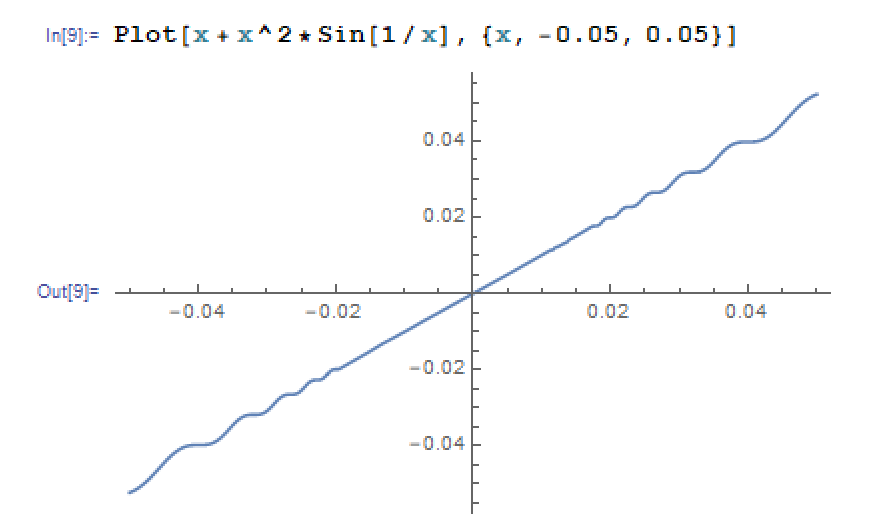
\includegraphics[scale=0.35]{f}
	\end{figure}
	
	We first show that $f$ is continuous. When $x\neq 0$, $f$ is clearly continuous. So we only focus on showing $f$ is continuous at $0$. Let $\epsilon > 0$ be given, then
	\begin{align*}
	\abs{f(x) - f(0)} = \abs{f(x)} \leq \abs{x} + \abs{2x^2 \sin\f{1}{x}} \leq \abs{x} + 2\abs{x^2}. 
	\end{align*}
	Choose $\delta = \min\{1, \epsilon/3\}$. Then whenever $\abs{x-0} < \delta$, we have
	\begin{align*}
	\abs{f(x) - f(0)} \leq \abs{x} + 2\abs{x^2} = \abs{x}(2\abs{x} + 1) < \f{\epsilon}{3}\cdot 3 < \epsilon.
	\end{align*}
	This shows $f$ is continuous. Next, we want to show $f'(0) > 0$. To this end, we just evaluate $f'(0)$. By definition,
	\begin{align*}
	f'(0) = \lim_{x\to 0} \f{f(x) - f(0)}{x-0} = \lim_{x\to 0 }\f{f(x)}{x} = \lim_{x\to 0} \left( 1 + 2x\sin\f{1}{x}\right)= 1 > 0
	\end{align*}
	since $x\sin(1/x) \to 0$ as $x\to 0$. Finally, we will show that $f$ is not increasing on any interval containing 0. Assume (to get a contradiction) that $f$ is increasing on some interval containing 0. Because $f'$ is continuous and positive at 0, there exists an interval containing 0 on which $f'>0$ (we proved this in the last item). Now, look at $f$ again. For $x\neq 0$, 
	\begin{align*}
	f'(x) = 1-2\cos\f{1}{x} + 4x\sin\f{1}{x}.
	\end{align*}
	Let an interval containing $0$ be given. It is possible to find a sufficiently small $t$ in this interval such that $\cos(1/t) = 1$ and $\abs{4t} < 1/2$ (This is possible because $1/t$ will be sufficiently large in magnitude and $\cos$ is periodic.) It follows that
	\begin{align*}
	\abs{f'(t) + 1} = \abs{1-2 + 4t\sin\f{1}{t} + 1} = \abs{4t\sin\f{1}{t}} \leq \abs{4t} < 1/2,  
	\end{align*} 
	which implies $-3/2 < f(t) < -1/2$. Clearly, $f(t) < 0$, which contradicts the fact that there exists an interval containing 0 on which $f'(t) > 0$ for all $t$ on that interval.  \hfill $\square$
	
	
	
	
	
	
	
	
	
	
	
	
	
	
	
	
	
	
	\item Assume that $\abs{f(x) - f(y)} \leq (x-y)^2$ for all $x,y\in \mathbb{R}$. Prove that $f$ is a constant function. 
	
	
	
	\noindent \textit{\underline{Proof}:} Let $\delta > 0$ be given. Pick $x,y \in \mathbb{R}$ such that $0 < x-y< \delta$. Because $\abs{f(x) - f(y)} \leq (x-y)^2$ for all $x,y\in \mathbb{R}$, we have
	\begin{align*}
	0 \leq \f{\abs{f(x) - f(y)}}{x-y} = \abs{\f{f(x) - f(y)}{x-y}} \leq x-y < \delta.
	\end{align*}
	Since this holds for any $\delta > 0$, $f'(x) = 0$ for all $x\in\mathbb{R}$ (because $f'(x)$ is the limit of the difference quotient as $y\to x$). This means $f$ is constant, by Theorem 5.11(b), Baby Rudin. \hfill $\square$
\end{enumerate}






\newpage



\noindent \textbf{2. Series}

\begin{enumerate}[(a)]
	\item Prove that if $\sum^\infty_{n=1}a_n$ is absolutely convergent then 
	\begin{align*}
	\abs{\sum^\infty_{n=1}a_n} \leq \sum^\infty_{n=1}\abs{a_n}.
	\end{align*} 
	
	
	
	\noindent \textit{\underline{Proof}:} Since $\sum^\infty_{n=1}a_n$ converges absolutely, $\sum^\infty_{n=1}a_n$ converges (Theorem 3.45). Let $C = \sum^\infty_{n=1}a_n$. Consider the sequence $\{\abs{s_N}\}$ where each $s_N = {\lim^{N}_{n=1}a_n}$.  Clearly, 
	\begin{align*}
	\abs{\abs{s_N} - \abs{C}} \leq \abs{ s_N - C} \to 0, \mbox{ as } N\to \infty.
	\end{align*}
	Thus, $\lim_{N\to \infty}\abs{s_N} = \abs{C}$. Now, for each $N$, we also have the triangle inequality:
	\begin{align*}
	\abs{s_N} = \abs{\sum^N_{n=1}a_n} \leq \sum^N_{n=1}\abs{a_n}.
	\end{align*}
	Taking $N\to \infty$ on both sides we have
	\begin{align*}
	\lim_{N\to \infty}\abs{s_N} = \abs{C} =  \abs{\sum^\infty_{n=1}a_n} \leq \lim_{N\to \infty} \sum^N_{n=1}\abs{a_n} = \sum^\infty_{n=1}\abs{a_n}.
	\end{align*}
 	\hfill $\square$
	
	
	
	
	
	
	
	
	
	
	
	
	
	
	
	
	
	
	
	
	
	\item Show that if $\sum^\infty_{n=1}a_n$ is absolutely convergent and $b_n$ is a subsequence of $a_n$, then $\sum^\infty_{n=1}b_n$ is absolutely convergent. Given an example that shows this statement is false if $\sum^\infty_{n=1}a_n$ is assumed to be only conditionally convergent. 
	
	
	
	\noindent \textit{\underline{Proof}:} The absolute convergence of $\sum^\infty_{n=1}a_n$ implies the convergence of $\sum^\infty_{n=1}\abs{a_n}$. Since $b_n$ is a subsequence of $a_n$, we must have that
	\begin{align*}
	\sum^\infty_{n=1}\abs{b_n} \leq \sum^\infty_{n=1}\abs{a_n} < \infty, 
	\end{align*} 
	where the first inequality follows because we are summing only nonnegative terms. Therefore, $\sum^\infty_{n=1}b_n$ is absolutely convergent. 
	
	
	When $\sum^\infty_{n=1}a_n$ is assumed to be only conditionally convergent, that is $\sum^\infty_{n=1}\abs{a_n}$ is divergent, then the statement is false. Consider the conditionally convergent series $\sum^\infty_{n=1}(-1)^{n+1}/n$:
	\begin{align*}
	\sum^\infty_{n=1}(-1)^{n+1}/n = 1 - \f{1}{2} + \f{1}{3} - \f{1}{4} + \dots
	\end{align*}
	We know that $\sum^\infty_{n=1}1/n$ is divergent (harmonic series). Call $a_n = (-1)^{n+1}/n$. Clearly, $\abs{a_1}\geq \abs{a_2} \geq \dots$; the sequence $\{a_n\}$ is alternating; and $\lim_{n\to \infty} a_n = 0$. Theorem 3.43 (alternating series test) tells us that $\sum^\infty_{n=1}(-1)^{n+1}/n$ is convergent. Hence, $\sum^\infty_{n=1}(-1)^{n+1}/n$ is conditionally convergent. 
	
	Consider the subsequence $\{b_n\}$ of $\{a_n\}$ consisting only of the terms of $a_n$ where $n$ is odd:
	\begin{align*}
	\sum^\infty_{n=1}b_n = 1 + \f{1}{3} + \f{1}{5} + \f{1}{7} + \dots
	\end{align*}
	We want to show that the series $\sum^\infty_{n=1}b_{n}$ is NOT absolutely convergent. We notice that
	\begin{align*}
	\sum^\infty_{n=1}\abs{b_n} = \sum^\infty_{n=1}b_n = 1 + \f{1}{3} + \f{1}{5} + \f{1}{7} + \dots = \sum^\infty_{n=1}\f{1}{2n-1}
	\end{align*}
	So this comes down to determining the convergence of $\sum^\infty_{n=1} b_n$. It turns out that $\sum^\infty_{n=1}b_n > \infty$ because it fails the integral test:
	\begin{align*}
	\int_1^\infty \f{1}{2n-1}\,dn = \lim_{k\to \infty}\int^k_1 \f{1}{2n-1}\,dn = \f{1}{2}\ln (1+2k) \to \infty
	\end{align*}
	as $k\to \infty$. Thus, $\sum^\infty_{n=1}b_n$ is NOT absolutely convergent. Therefore, the statement is false when $\sum^\infty_{n=1}a_n$ is only conditionally convergent. \hfill $\square$ 	
	
	
	
	
	
	
	
	
	
	
	
	
	
	
	
	
	
	
	 
	\item Assume $a_n$ is a decreasing sequence of positive numbers, and that $\sum^\infty_{n=1}a_n$ converges. Prove that $\lim_{n\to \infty}na_n = 0$.
	
	\noindent \textit{\underline{Proof}:} The key here is to put an upper bound on $na_n$ and show that bound goes to zero as $n\to \infty$. Consider the partial sum $S_n = \sum^{n}_{i=1}a_i$. We have
	\begin{align}
	S_{2n} - S_n &= \sum_{i={n+1}}^{2n} = a_{2n} + a_{2n-1} + \dots + a_{n+1}\\
	&\geq a_{2n} + a_{2n} + \dots + a_{2n}\\
	&= na_{2n}.
	\end{align}
	where we have used the condition that $a_n$ is a decreasing sequence of positive numbers to get the inequality. Now, $\sum^\infty_{n=1}a_n$ is convergent, so the sequence of partial sums is convergent, hence Cauchy. It follows that for any $\epsilon > 0$, there exists $N \in \mathbb{N}$ such that whenever $n \geq N$, 
	\begin{align*}
	\abs{na_{2n}} \leq \abs{S_{2n} - S_n} = \abs{\sum_{i={n+1}}^{2n}} < \epsilon.
	\end{align*}
	Thus $\lim_{n\to\infty} na_{2n} = 0$ and so $\lim_{n\to \infty}2na_{2n} = 0$. Further,
	\begin{align*}
	(2n+1)a_{2n+1} \leq (2n+1)a_{2n} = \left(1 + \f{1}{2n}\right)(2na_n) \leq 2\cdot 2na_{2n} = 4na_{2n},
	\end{align*}
	which also goes to 0 as $n\to \infty$. So, because both $na_{n} \to 0$ as $n\to \infty$ for all $n$ (odd or even), $\lim_{n\to \infty} na_n = 0$. \hfill$\square$
	
	
	
	
	
	
	
	
	
	
	
	
	
	
	
	
	 
	\item Prove that every positive rational number can be written as a finite sum of \textit{distinct} numbers of the form $1/k$ with $k\in \mathbb{N}$.
	
	
	
	\noindent \textit{\underline{Proof}:} We will first show this is true for all rationals $r$ such that $0 \leq r=p/q < 1$ where $p,q$ are positive integers with no common factor. If $r=0$ or $p=1$ then the statement is true. Assume (an inductive hypothesis) that the statement holds for all rationals $r$ above but with $p<P$. Consider the rational number $P/q < 1$. We can always find the least positive integer $m$ such that $1/m \leq P/q$. Because $P/q < 1$ and $m$ is an integer, we have 
	\begin{align*}
	\f{1}{m} \leq \f{P}{q} < \f{1}{m-1} \implies mP - P < q \leq mP \implies 0 \leq mP-q < P.
	\end{align*}  
	Let the residual $R = P/q - 1/m = (mP-q)/qm$. Because $mP -q < P$, $R$ can be written as a finite sum of distinct $1/k$'s, $k\in \mathbb{N}$. We also have that 
	\begin{align*}
	R < \f{1}{m-1} - \f{1}{m} = = \f{1}{m(m-1)} \leq \f{1}{m}.
	\end{align*} 
	So, $1/m$ cannot appear in the finite sum for $R$. This means $r = P/q = R + 1/m$ can be written as a finite sum of distinct $1/k$'s. By induction, all rationals less than 1 can be written as a finite sum of distinct $1/k$'s, $k\in \mathbb{N}$. 
	
	We now want to extend this to all rationals greater than or equal to 1. We now use the fact that $\sum^\infty_{n=1}1/n = \infty$. Let $S_n = \sum^n_{i=1}1/i$, which is rational. Let a rational $r \geq 1$ be given. There exists $n\in \mathbb{N}$ such that 
	\begin{align*}
	S_{n} \leq r < S_{n+1}.
	\end{align*}
	Now let us write $r = (r - S_n) + S_n$, which is a sum of two rational numbers. By the choice of $n$,
	\begin{align*}
	r - S_n < S_{n+1} - S_n = \f{1}{n+1} < 1,
	\end{align*} 
	which means $r - S_n$ can be written as a finite sum of distinct $1/k$'s, $k\in \mathbb{N}$. Further, none of the summands in the sum for $r - S_n$ is can be greater than $1/(n+1)$, which means no summand in the sum for $r-S_n$ can be a summand of $S_n$, which is a finite sum of distinct $1/k$'s, $k\in \mathbb{N}$. Therefore, $r$ can be written as a finite sum of distinct numbers of the form $1/k$ with $k \in \mathbb{N}$. \hfill $\square$
	
 	
	 
\end{enumerate}




\newpage









\noindent \textbf{3. Hilbert Space}

\begin{enumerate}[(a)]
	\item Let $V$ denote the set of continuous functions that map $[0,1]$ into the complex numbers $\mathbb{C}$. With $f\in V$, each complex number $f(x)$ can be written in terms of its real and imaginary parts
	\begin{align*}
	f(x) = \Re{f(x)} + i\Im{f(x)}.
	\end{align*}
	The real valued functions $\Re{f}$ and $\Im{f}$ are called the real part of $f$ and the imaginary part of $f$, respectively. We define the integral of a complex valued function by 
	\begin{align*}
	\int^1_0 f(x)\,dx \equiv \int^1_0 \Re{f(x)}\,dx + i\int^1_0\Im{f(x)}\,dx.
	\end{align*}
	Show that the assignment 
	\begin{align*}
	\langle f,g \rangle \equiv \int^1_0 f(x)\overline{g(x)}\,dx
	\end{align*}
	satisfies the axioms of a complex inner product (find the axioms in a book or on the internet).
	
	
	
	
	
	
	
	
	\noindent \textit{\underline{Proof}:} Let $f,g,h\in V$ and $c\in \mathbb{C}$ be given. From MA352: Complex Analysis, we know that the real and imaginary part of a continuous complex-valued function on $[0,1]$ are also continuous on $[0,1]$. This means if $f\in V$ then $\Re{f}, \Im{f} \in V$. Since products and sums of continuous functions on $[0,1]$ are also continuous on $[0,1]$. Further, the complex conjugate of a continuous function on $[0,1]$ is also a continuous function on $[0,1]$, so if $f,g\in V$ then $f\overline{g}\in V$. Now we're ready to show the axioms of a  complex inner product are satisfied. 
	
	\begin{itemize}
		\item $\boxed{\langle f,g \rangle = \overline{\langle g,f\rangle}}$. We have that
		\begin{align*}
		\langle f,g \rangle \equiv \int^1_0 f(x)\overline{g(x)}\,dx
		\end{align*}
		and
		\begin{align*}
		g(x)\overline{f(x)} &= \left[\Re{g(x)} + i\Im{g(x)}\right]\left[\Re{f(x)} - i\Im{f(x)}\right]\\
		&= \left[\Re{f(x)}\Re{g(x)} + \Im{f(x)}\Im{g(x)}\right] \\
		&\qquad + i\left[\Im{g(x)}\Re{f(x)} - \Re{g(x)}\Im{f(x)}\right],
		\end{align*}
		\begin{align*}
		f(x)\overline{g(x)} &= \left[\Re{f(x)} + i\Im{f(x)}\right]\left[\Re{g(x)} - i\Im{g(x)}\right]\\
		&= \left[\Re{g(x)}\Re{f(x)} + \Im{g(x)}\Im{f(x)}\right] \\
		&\qquad + i\left[\Im{f(x)}\Re{g(x)} - \Re{f(x)}\Im{g(x)}\right].
		\end{align*}
		So, $\Re{g(x)\overline{f(x)}} = \Re{f(x)\overline{g(x)}}$ and $\Im{g(x)\overline{f(x)}} = -\Im{f(x)\overline{g(x)}}$
		\begin{align*}
		\overline{\langle g,f \rangle} &= \overline{\int^1_0 g(x)\overline{f(x)}\,dx}\\
		&= \overline{\int^1_0 \Re{g(x)\overline{f(x)}}\,dx + i\int^1_0 \Im{g(x)\overline{f(x)}}\,dx}\\
		&= \int^1_0 \Re{g(x)\overline{f(x)}}\,dx - i\int^1_0 \Im{g(x)\overline{f(x)}}\,dx\\
		&= \int^1_0 \Re{f(x)\overline{g(x)}}\,dx + i\int^1_0 \Im{f(x)\overline{g(x)}}\,dx\\
		&= \int^1_0 f(x)\overline{g(x)}\,dx \\
		&= \langle f,g\rangle.
		\end{align*}
		
		
		
		
		
		\item $\boxed{\langle f+g ,h \rangle  = \langle f,h \rangle + \langle g,h\rangle}$. Since $f,g,h\in V$, we have that $(f+g\overline{h}) = f\overline{h} + g\overline{h} \in V$. This means $(f+g)\overline{h}, f\overline{h}, g\overline{h}$, and their respective real and imaginary parts are Riemann-integrable on $[0,1]$ (Theorem 6.8). With this, we can use the usual (linear) properties of the integral (Theorem 6.12):
%		We have that 
%		\begin{align*}
%		\Re{(f+g)\overline{h}} = \Re{f\overline{h} + g\overline{h}} =\Re{f\overline{h}} + \Re{g\overline{h}}\\
%		\Im{(f+g)\overline{h}} = \Im{f\overline{h} + g\overline{h}} =\Im{f\overline{h}} + \Im{g\overline{h}}
%		\end{align*}
%		So,
%		\begin{align*}
%		\langle f+g,h\rangle &= \int^1_0 (f+g)\overline{h}\,dx \\
%		&= \int^1_0 \Re{(f+g)\overline{h}}\,dx + i\int^1_0 \Im{(f+g)\overline{h}}\,dx\\
%		&= \int^1_0 \Re{f\overline{h}} + \Re{g\overline{h}}\,dx + i\int^1_0 \Im{f\overline{h}} + \Im{g\overline{h}}\,dx\\ 
%		&= \int^1_0 \Re{f\overline{h}}\,dx + i\int^1_0\Im{f\overline{h}} \,dx  + \int^1_0 \Re{g\overline{h}}\,dx + i\int^1_0\Im{g\overline{h}} \,dx \\
%		&= \int^1_0 f\overline{h}\,dx + \int^1_0 g\overline{h}\,dx\\
%		&=\langle f,h\rangle + \langle g,h\rangle.
%		\end{align*}
		\begin{align*}
		\langle f+g,h\rangle &= \int^1_0 (f+g)\overline{h}\,dx\\
		&= \int^1_0 f\overline{h} + g\overline{h}\,dx\\
		&= \int^1_0 f\overline{h}\,dx + \int^1_0 g\overline{h}\,dx\\
		&= \langle f,h\rangle + \langle g,h\rangle.
		\end{align*}
		
		
		\item $\boxed{\langle f, g+h \rangle  = \langle f,g \rangle + \langle f,h\rangle}$. Here we use the fact that $\overline{g+h} = \overline{g} + \overline{h}$:
		\begin{align*}
		\langle f, g+h\rangle &= \int^1_0 f\overline{(g+h)}\,dx\\
		&= \int^1_0 f\overline{g} + f\overline{h}\,dx\\
		&= \int^1_0 f\overline{g}\,dx + \int^1_0 f\overline{h}\,dx\\
		&= \langle f,g\rangle + \langle f,h\rangle.
		\end{align*}
		
		
		\item $\boxed{\langle cf,g\rangle = c\langle f,g\rangle}$. This follows from one of the properties of the integral:
		\begin{align*}
		\langle cf, g\rangle = \int^1_0 cf\overline{g}\,dx = c\int^1_0 f\overline{g}\,dx= c\langle f,g\rangle.
		\end{align*}
		
		\item $\boxed{\langle f,cg\rangle = \overline{c}\langle f,g\rangle}$. This also follows from one of the properties of the integral:
		\begin{align*}
		\langle f, cg\rangle = \int^1_0 f\overline{cg}\,dx = \int^1_0 f\overline{c}\overline{g}\,dx = \overline{c}\int^1_0 f\overline{g}\,dx = \overline{c}\langle f,g\rangle.
		\end{align*}
		
		\item $\langle f,f\rangle$ is a nonnegative real number and $\langle f,f \rangle = 0$ if and only if $f=0$.
		\begin{enumerate}[(i)]
			\item $\langle f,f\rangle$ is a nonnegative real number. First,
			\begin{align*}
			\langle f,f\rangle = \overline{\langle f,f\rangle}
			\end{align*}
			since the first axiom is satisfied. This means $\langle f,f\rangle$ is a real number. Next, suppose $f$ is a continuous function on $[0,1]$, then $f^2$ is also a continuous function on $[0,1]$. With this, we proceed:
			\begin{align*}
			\langle f,f\rangle =  \int^1_0  f\overline{f}\,dx &= \int^1_0 \left(\Re{f} + i\Im{f}\right)\left(\Re{f} - i\Im{f}\right) \,dx\\
			&= \int^1_0 \left(\Re{f}\right)^2 + \left(\Im{f}\right)^2\,dx.
			\end{align*}
			Now, the integrand is a continuous, nonnegative, real-valued function on $[0,1]$ (hence integrable on $[0,1]$). So we have, by Theorem 6.13, 
			\begin{align*}
			\langle f,f\rangle 
			= \int^1_0 \left(\Re{f}\right)^2 + \left(\Im{f}\right)^2\,dx&= \int^1_0 \abs{\left(\Re{f}\right)^2 + \left(\Im{f}\right)^2}\,dx \\
			&\geq \abs{\int^1_0 \left(\Re{f}\right)^2 + \left(\Im{f}\right)^2\,dx} \\
			&\geq 0.
			\end{align*} 
			So, $\langle f,f\rangle$ is a nonnegative real number. 
			
			
			
			
			\item $\langle f,f \rangle = 0$ if and only if $f=0$: If $f =0$ then 
			\begin{align*}
			\langle f,f\rangle = \int^1_0 0\,dx= 0.
			\end{align*}
			If $\langle f,f\rangle = 0$ then 
			\begin{align*}
			\int^1_0 \left(\Re{f}\right)^2 + \left(\Im{f}\right)^2\,dx = 0 \iff \Re{f} = \Im{f} = 0 \iff f=0.
			\end{align*}
		Note that we don't worry about the case where $f$ can be zero almost everywhere because $f$ is continuous on $[0,1]$. 
		 
		\end{enumerate}
		\hfill$\square$ 	

	
	

	 
		
	
	\end{itemize}  
	
	
	
	\newpage
	
	
	
	
	
	\item Assume $V$ is a complex inner product space with inner product $\langle x,y \rangle$ and its associated metric
	\begin{align*}
	d(x,y) = \sqrt{\langle x-y,x-y \rangle}
	\end{align*}
	and let $\mathcal{H}$ denote the metric completion of $V$. Thus we may think of $V$ as a dense subset of the metric space $\mathcal{H}$. The purpose of the following exercises is to show how one may extend the vector space structure of $V$ to $\mathcal{H}$, and how to extend the inner product to $\mathcal{H}$, which shows that the metric completion of an inner product space is a Hilbert space. 
	
	
	\begin{itemize}
		\item Given $x,y\in \mathcal{H}$ and $\alpha,\beta \in \mathbb{C}$, we define $\alpha x + \beta y$ to be the limit of the sequence $\alpha x_i + \beta y_i$, where $x_i$ is any sequence in $V$ converging to $x$, $y_i$ is any sequence in $V$ converging to $y$. Show that this definition is well-defined. 
		
		
		\noindent \textit{\underline{Proof}:} First, we call Cauchy the sequence $\{y_n\}$ in $V$ equivalent to another Cauchy sequence $\{x_n\}$ in $V$ if $ \lim_{n\to \infty}d(y_n,x_n) =0$. This establishes an equivalence relation:
		\begin{itemize}
			\item \textit{Reflexivity:} $d(x_n,x_n) = \sqrt{\langle x_n-x_n,x_n-x_n\rangle} = \sqrt{\langle 0,0 \rangle} =0$ for all $n$, so $\lim_{n\to \infty} d(x_n,x_n) = 0$, which means $\{x_n\}$ is equivalent to itself. 
			\item \textit{Symmetry:} Suppose $\{y_n\}$ is equivalent to $\{x_n\}$, then because 
			\begin{align*}
			d(y_n,y_n) = \sqrt{\langle y_n -x_n, y_n-x_n\rangle} = \sqrt{\langle x_n-y_n, x_n-y_n \rangle} = d(x_n,y_n),
			\end{align*}
			we have $\lim_{n\to \infty} d(y_n,x_n) = \lim{n\to \infty} d(x_n,y_n) = 0$, so $\{x_n\}$ is equivalent to $\{y_n\}$. 
			\item \textit{Transitivity:} If $\{x_n\}$ is equivalent to $\{y_n\}$ and $\{y_n\}$ is equivalent to $\{z_n\}$ then because $
			d(x_n,z_n) \leq d(x_n,y_n) + d(y_n , z_n)$
			(since $d(x,y)$ defines a metric on $V$), and because $\lim_{n\to \infty}d(x_n,y_n) = 0 = \lim_{n\to\infty}d(y_n,z_n)$, we have that $\lim_{n\to \infty}d(x_n,z_n) = 0$ as well, by comparison test. So, $\{x_n\}$ is equivalent to $\{z_n\}$.   
		\end{itemize}
		$\mathcal{H}$ is the metric completion of $V$, so it is the set of all equivalence classes obtained above. If $X \in \mathcal{H}$ and $Y\in \mathcal{H}$ and $\{x_n\} \in X, \{y_n\}\in Y$ , then $
		\Delta (X,Y) = \lim_{n\to \infty}d(x_n,y_n)$ defines a distance function in $\mathcal{H}$ (the proof is similar to that in Exercise 24(b), Chapter 3, Baby Rudin).
		
		Now, we define $\alpha x + \beta y$ to be the limit of $\{\alpha x_i + \beta y_i\}$ for $x_i \to x$ and $y_i \to y$, i.e., $\{x_i\}\in X$ and $\{ y_i\} \in Y$. To show that this definition is well-defined, we want to show that the sequences $\{\alpha x_i + \beta y_i\}$ is equivalent to the sequence $\{ \alpha u_i + \beta v_i \}$, provided that $\{x_i\}, \{u_i\} \in X$ and $\{y_i\}, \{v_i\} \in Y$. To this end, we want to show 
		\begin{align*}
		\lim_{i\to\infty} d(\alpha x_i + \beta y_i , \alpha u_i + \beta v_i) = 0.
		\end{align*}
		From our definition of the distance function $\Delta$ above, we have
		\begin{align*}
		\lim_{n\to \infty}d(\alpha x_i + \beta y_i, \alpha u_i + \beta v_i) = \Delta(\alpha X + \beta Y, \alpha X + \beta Y) = 0.
		\end{align*}
		\hfill$\square$ 
		
		
		
		
		
		
		
		
		
		
		
		
		
		
		
		
		\item Imitate the procedure above to show how to extend the inner product so that $\langle x,y\rangle$ is defined for all $x,y\in \mathcal{H}$. (Hint: extend one variable at a time.)
		
		
		\noindent \textit{\underline{Proof}:} Now, we will let $\langle \cdot,\cdot \rangle_V$ denote the inner product in $V$ and $\langle  \cdot, \cdot \rangle_\mathcal{H}$ denote the inner product in $\mathcal{H}$, which we will define as an extension of $\langle \cdot, \cdot \rangle_V$. We will try to extend in one variable at a time. Let $\{x_i\} \in X \in \mathcal{H}$ and $\{y_i\} \in Y \in \mathcal{H}$ be given. We define 
		\begin{align*}
		\langle X,Y\rangle_\mathcal{H} = \lim_{i\to \infty}\langle x_i, y_i\rangle_V.
		\end{align*}
		We will first show that the limit on the right hand side exists. Then we will show that this definition is well defined. Finally, we will show that this definition gives an inner product on $\mathcal{H}$. 
		
		To prove: $\lim_{i\to\infty}\langle x_i,y_i \rangle$ exists. Let $\{x_i\}$ and $\{y_i\}$ be Cauchy sequences in $V$. Then we have
		\begin{align*}
		\abs{\langle x_n,y_n\rangle_V - \langle x_m,y_m\rangle_V} &= \abs{\langle x_n,y_n \rangle_V - \langle x_n, y_m\rangle_V + \langle x_n,y_m \rangle_V - \langle x_m,y_m \rangle_V}\\
		&= \abs{\langle x_n, y_n -y_m \rangle_V  + \langle x_n-x_m, y_m \rangle_V }\\
		&\leq \abs{\langle x_n, y_n -y_m \rangle_V} + \abs{\langle x_n-x_m, y_m \rangle_V}\\
		&\leq \norm{x_n}_V\norm{y_n-y_m}_V + \norm{y_m}_V\norm{x_n - x_m}_V 
		\end{align*}
		where 
		\begin{align*}
		\norm{x_n}_V = \sqrt{\abs{\langle x_n,x_n\rangle_V}} = d(x,0)
		\end{align*}
		and the last inequality is the Cauchy-Schwarz inequality:
		\begin{align*}
		\abs{\langle x,y\rangle_V}  \leq \sqrt{\abs{\langle x,x\rangle_V}}\sqrt{\abs{\langle y,y\rangle_V}}= \norm{x}_V \norm{y}_V.
		\end{align*}
		Since $\{x_i\}$ and $\{y_i\}$ are Cauchy sequences, they are bounded. Thus, there exists some $M > 0$ such that for all $m,n$ 
		\begin{align*}
		\abs{\langle x_n,y_n\rangle_V - \langle x_m,y_m\rangle_V} \leq M\left( \norm{y_n-y_m}_V + \norm{x_n - x_m}_V \right).
		\end{align*}
		By the Cauchy-ness of $\{y_i\}$ and $\{x_i\}$, when given any $\epsilon > 0$,  there are $m,n$ are sufficiently large such that
		\begin{align*}
		\abs{\langle x_n,y_n\rangle_V - \langle x_m,y_m\rangle_V}  \leq M\left( \norm{y_n-y_m}_V + \norm{x_n - x_m}_V \right) < \epsilon.
		\end{align*}
		This means $\{ \langle x_i, y_i\rangle_V \}$ is a Cauchy sequence in $\mathbb{R}$. Since $\mathbb{R}$ is complete, $\{ \langle x_i, y_i\rangle_V \}$ converges, and thus $\lim_{i\to \infty}\langle x_i, y_i\rangle_V$ exists. 
		
		
		Now, we want to show that the definition 
		\begin{align*}
		\langle X,Y\rangle_\mathcal{H} = \lim_{i\to \infty}\langle x_i, y_i\rangle_V.
		\end{align*}
		is well-defined. Let $\{x_i\}, \{u_i\} \in X$, i.e., $\{x_i\}$ and $\{u_i\}$ are equivalent, and $\{y_i\}, \{ v_i\} \in Y$. Then
		\begin{align*}
		\abs{\langle x_n,y_n\rangle_V - \langle u_n,v_n\rangle_V} &= \abs{\langle x_n,y_n \rangle_V - \langle x_n, v_n\rangle_V + \langle x_n,v_n \rangle_V - \langle u_n,v_n \rangle_V}\\
		&= \abs{\langle x_n, y_n -v_n \rangle_V  + \langle x_n-u_n, y_m \rangle_V }\\
		&\leq \abs{\langle x_n, y_n -v_n \rangle_V} + \abs{\langle x_n-u_n, y_m \rangle_V}\\
		&\leq \norm{x_n}_V\norm{y_n-v_n}_V + \norm{v_n}_V\norm{x_n - u_n}_V .
		\end{align*}
		Again, $\{v_i\}$ and $\{x_i\}$ are bounded and the fact that $\lim_{i\to\infty}d(y_i,v_i) = 0 = \lim_{i\to\infty}d(x_i,u_i)$, we have
		\begin{align*}
		\lim_{i\to \infty}\langle x_i,y_i\rangle_V = \lim_{i\to\infty}\langle u_i,v_i \rangle_V.
		\end{align*}
		This says that the number $\langle X,Y\rangle_\mathcal{H}$ is unchanged when we picked different representatives for $X,Y$, i.e., the definition $\langle x,y\rangle_\mathcal{H} = \lim_{n\to\infty}\langle x_n,y_n\rangle_V$ is well-defined. 
		
		
		Finally, we want to show that $\langle X,Y\rangle_{\mathcal{H}}$ defines an inner product. To this end, we once again check that $\langle \cdot,\cdot\rangle_\mathcal{H}$ satisfies the axioms for complex inner products. This is more straightforward because a lot of these properties carry over from the inner product in $V$:
		\begin{enumerate}[(i)]
			\item Let $\{x_n\} \in X$ and $\{y_n\} \in Y$ be given. $X,Y\in \mathcal{H}$:
 			\begin{align*}
			\langle X,Y \rangle_\mathcal{H} = \lim_{n\to \infty}\langle x_n,y_n \rangle_V = \lim_{n\to \infty}\overline{\langle y_n,x_n \rangle_V} = \overline{\lim_{n\to \infty}{\langle y_n,x_n \rangle_V}} = \overline{\langle Y,X\rangle_\mathcal{H}}.
			\end{align*}
			
			\item Let $\{x_n\} \in X$, $\{y_n\} \in Y$, and $\{z_n\} \in Z$ be given. $X,Y,Z\in \mathcal{H}$:
			\begin{align*}
			\langle X+Y,Z \rangle_\mathcal{H} &= \lim_{n\to\infty}\langle x_n+y_n,z_n \rangle_V \\
			&= \lim_{n\to\infty}\left(\langle x_n,z_n \rangle_V + \langle x_n,y_n\rangle_V\right) \\
			&= \lim_{n\to\infty}\langle x_n,z_n \rangle_V + \lim_{n\to\infty}\langle x_n,y_n\rangle_V\\
			&= \langle X,Z \rangle_\mathcal{H} + \langle X,Y\rangle_\mathcal{H} 
			\end{align*}
			which follows from the fact that $\lim_{n\to\infty}\langle x_n,y_n \rangle_V$ exists for all Cauchy sequences $\{x_n\}, \{y_n\}$ in $V$.
			
			\item Similarly,
			\begin{align*}
			\langle X,Y+Z\rangle_\mathcal{H} = \langle X,Y\rangle_\mathcal{H} + \langle X,Z\rangle_\mathcal{H}.
			\end{align*}
			
			\item Let a constant $c\in \mathbb{C}$ be given
			\begin{align*}
			\langle cX,Y\rangle_\mathcal{H} = \lim_{n\to\infty}\langle cx_n,y_n\rangle_V = c \lim_{n\to\infty}\langle x_n,y_n\rangle_V = c\langle X,Y\rangle_\mathcal{H}.
			\end{align*}

			
			
			\item Let a constant $c\in \mathbb{C}$ be given
			\begin{align*}
			\langle X,cY\rangle_\mathcal{H} = \lim_{n\to\infty}\langle x_n,cy_n\rangle_V = \overline{c} \lim_{n\to\infty}\langle x_n,y_n\rangle_V = \overline{c}\langle X,Y\rangle_\mathcal{H}.
			\end{align*}
			
			
			\item 
			\begin{align*}
			\langle X,X\rangle_\mathcal{H} = \lim_{n\to \infty}\langle x_n,x_n\rangle_V = \lim_{n\to\infty}\norm{x_n}^2.
			\end{align*}
			Since $\{x_n\}$ is Cauchy (hence bounded), the limit exists and is a nonnegative real number. So, $\langle X,X\rangle_\mathcal{H}$ is a nonnegative real number. 
			
			
			If $X = 0$, then 
			\begin{align*}
			\langle X,X\rangle_{\mathcal{H}} = \lim_{n\to\infty}\langle x_n,x_n \rangle_V = \langle 0,0\rangle_V = 0.
			\end{align*}
			If $\langle X,X\rangle_\mathcal{H} = 0$ then 
			\begin{align*}
			\langle X,X\rangle_\mathcal{H} =\lim_{n\to\infty}\langle x_n,x_n\rangle_V = \lim_{n\to\infty} (d(x_n,0))^2 =  0,
			\end{align*}
			which implies 
			\begin{align*}
			\lim_{n\to\infty}d(x_n,0) = 0,
			\end{align*}
			so $\{x_n\} \to 0$. Thus, $X = 0$.
		\end{enumerate}		
	\hfill$\square$
		
		
		
		
		
		
		
		
		
		
		
		
		
		
	\end{itemize}
\end{enumerate}



\newpage








\noindent \textbf{4. Isometries}

\begin{enumerate}[(a)]
	\item Assume that $f: \mathbb{R} \to \mathbb{R}$ satisfies $\abs{f(x) - f(y)} = \abs{x-y}$ for all $x,y\in \mathbb{R}$. Prove that 
	\begin{align*}
	f(x) = mx+b
	\end{align*}
	with $m=1$ or $m=-1$.
	
	\noindent \textit{\underline{Proof}:} For any $\epsilon > 0$, there exists $\delta = \epsilon$ such that whenever $\abs{x-y} < \delta$, $\abs{f(x) - f(y)} < \epsilon$. So $f$ is continuous at all $x\in \mathbb{R}$. Further, for any $x\neq y$
	\begin{align*}
	\f{\abs{f(x) - f(y)}}{\abs{x-y}} = 1
	\end{align*}
	which implies 
	\begin{align*}
	\lim_{x\to y}\f{f(x) - f(y)}{x-y} = \pm 1.
	\end{align*}
	So, $f$ is differentiable at all $x\in \mathbb{R}$, with $f'(x) = \pm 1$. If $f'(x) = 1$ then $f(x) = x+b$ for some constant $b\in \mathbb{R}$. If $f'(x) = -1$ then $f(x) = -x+b$ for some constant $b\in \mathbb{R}$. So, $f(x) = mx+b$ with $m=1$ or $m=-1$.\hfill$\square$
	
	
	
	
	
	
	
	\item Prove that there does not exist a function $f: \mathbb{R}^2 \to \mathbb{R}$ that satisfies $\abs{f(x) - f(y)} = \norm{x-y}$ for all $x,y\in \mathbb{R}^2$.
	
	
	
	\noindent \textit{\underline{Proof}:} Suppose such a function $f$ exists. Consider 3 distinct points $x,y,z\in \mathbb{R}^2$ such that $\norm{x-y} = \norm{y-z} = \norm{z-x} = 1$. Our assumption about $f$ tells us that 
	\begin{align*}
	\abs{f(x)-f(y)} = \abs{f(y) - f(z)} = \abs{f(z) - f(x)}=1.
	\end{align*} 
	Now, because $f(x),f(y),f(z)$ are three points in $\mathbb{R}$, this cannot happen: if $\abs{f(x) - f(y)} = \abs{f(y) -f(z)} = 1$, we must have that $f(z) = f(x)$ or $f(z) = f(x) \pm 2$. In either case $\abs{f(x) - f(z)}\neq 1$. So, no such function $f$ exists. \hfill$\square$ 
	
	
	
	
	
	
	
	
	
	
	
	
	
	
	
	\item Prove that if $f: \mathbb{R}^n \to \mathbb{R}^n$ satisfies $\norm{f(x) - f(y)} = \norm{x-y}$ for all $x,y\in \mathbb{R}^n$ then $f$ is onto.
	
	
	\noindent \textit{\underline{Proof}:} Without loss of generality, let us assume that $f(0) = 0$. So that $\norm{f(x)} = \norm{x}$ for all $x\in \mathbb{R}^n$. We will prove that $f$, in this case, is \textit{linear}, using the usual Euclidean inner product $\langle \cdot, \cdot \rangle$ defined by
	\begin{align*}
	\langle x,y\rangle = \sum^n_{i=1}x_iy_i
	\end{align*}
	for $x = (x_1,x_2,\dots,x_n)^\top \in \mathbb{R}^n$ and $y = (y_1,y_2,\dots,y_n)\in \mathbb{R}^n$. From this definition we have that for $x\in \mathbb{R}^n$,
	\begin{align*}
	\norm{x}^2 = \langle x,x\rangle.
	\end{align*}
	The inner product satisfies the axioms for real inner product. Further, the function $f$ preserves this inner product. We can show this via the polarization identity:
	\begin{align*}
	\langle x,y\rangle = \f{1}{4}\left( \norm{x+y}^2 - \norm{x-y}^2  \right).
	\end{align*}
	Because $\norm{f(x)-f(y)} =\norm{x-y}$, we have
	\begin{align*}
	\langle f(x),f(y)\rangle &= \f{1}{4}\left( \norm{f(x)+f(y)}^2 - \norm{f(x)-f(y)}^2  \right)\\
	&= \f{1}{4}\left( \norm{x+y}^2 - \norm{x-y}^2  \right)\\
	&= \langle x,y\rangle.
	\end{align*}
	With this, we are ready to show $f$ is linear. To this end, we want to show:
	\begin{itemize}
		\item $f(u+v) = f(u) + f(v)$.
		\item $f(\alpha u) = \alpha f(u)$, $\alpha \in \mathbb{R}$. 
	\end{itemize}
	
	First, we will show $f(u+v) = f(u) + f(v)$:
	\begin{align*}
	\norm{ f(u+v) - f(u) - f(v)}^2 
	&= \langle f(u+v) - f(u) - f(v), f(u+v) - f(u) - f(v)\rangle\\
	&= \norm{f(u+v)}^2 + \norm{f(u)}^2 + \norm{f(v)}^2 \\
	&\qquad- 2\langle f(u+v),f(u)\rangle -2\langle f(u+v),f(v)\rangle +2\langle f(u),f(v) \rangle\\
	&= \norm{u+v}^2 + \norm{u}^2 + \norm{v}^2 -2\langle u+v,u+v\rangle +2\langle u,v\rangle\\
	&=\langle u+v -u-v, u+v-u-v\rangle\\
	&= \norm{(u+v) - u- v}^2\\
	&= 0.
  	\end{align*}   
	This holds if and only if $f(u+v) = f(u) + f(v)$.
	
	
	Next, we want to show $f(\alpha u) = \alpha f(u)$ for $\alpha \in \mathbb{R}$:
	\begin{align*}
	\norm{\alpha f(u) - f(\alpha u)}^2 &= \langle \alpha f(u) - f(\alpha u), \alpha f(u) - f(\alpha u)  \rangle\\
	&= \norm{\alpha f(u)}^2 + \norm{f(\alpha u)}^2 -2\langle \alpha f(u),f(\alpha u) \rangle  \\
	&= \norm{\alpha u}^2 + \norm{\alpha u}^2 -2 \alpha\langle  f(u),f(\alpha u) \rangle \\
	&= \norm{\alpha u}^2 + \norm{\alpha u}^2 -2 \alpha\langle  u,\alpha u \rangle \\
	&= \norm{\alpha u}^2 + \norm{\alpha u}^2 -2 \langle \alpha u,\alpha u \rangle \\
	&= \norm{\alpha u}^2 + \norm{\alpha u}^2 -2\norm{\alpha u}^2 \\
	&= 0.
	\end{align*}
	This holds if and only if $\alpha f(u) = f(\alpha u)$. 
	
	
	Thus, we have shown that if $f(0) = 0$ and $f$ is an isometry, then $f$ is linear. Now, $f: \mathbb{R}^n \to \mathbb{R}^n$ is injective because whenever $x\neq y$, $\norm{f(x) - f(y)} = \norm{x-y} \neq 0$ which implies $f(x)\neq f(y)$. So, $\ker{f} = \{0\}$. By the rank-nullity theorem, $\dim\left( \Im(f)\right) = n$, or $f(\mathbb{R}^n) = \mathbb{R}^n$, i.e., $f$ is surjective. Thus, any isometry $f: \mathbb{R}^n \to \mathbb{R}^n$ can be written as bijective linear map followed by a shift. Since a shift is surjective, $f$ is surjective. \hfill$\square$ 
	
	
	
	
	
	\item Let $\mathcal{H}$ denote an infinite dimensional (real or complex) Hilbert space. Given an example of a function $f: \mathcal{H} \to \mathcal{H}$ that satisfies 
	\begin{align*}
	\norm{f(x) - f(y)} = \norm{x-y}
	\end{align*} 
	for all $x,y\in \mathcal{H}$ but $f$ is \textit{not} onto. 
	
	
	
	
	\noindent \textit{\underline{Solution}:} Consider the Hilbert space $\ell^2 = \{x = (x_1,x_2,\dots): x_i \in \mathbb{C} \mbox{ and } \sum^\infty_{n=1}\abs{x_i}^2 < \infty  \} $ with the norm
	\begin{align*}
	\norm{x} = \sqrt{\sum^\infty_{i=1}\abs{x_i}^2}.
	\end{align*} 
	Let $f: \ell^2 \to \ell^2$ be defined by
	\begin{align*}
	f[(x_1,x_2,x_3,\dots)] = (0,x_1,x_2,x_3,\dots).
	\end{align*}
	We see that for $x,y\in \mathcal{H}$, 
	\begin{align*}
	\norm{f(x)-f(y)} = \sqrt{\sum^\infty_{i=1}\abs{x_i - y_i}^2} = \norm{x-y},
	\end{align*}
	so $f$ is an isometry. However, $f$ is not onto, because $f$ does not map any sequence to $\ell^2$ to any sequence that don't start with $0$ in $\ell^2$, such as $(1,1/2,1/4,1/8,\dots) \in \ell^2$. \hfill $\square$ 
	
	
	
	
	
\end{enumerate}




\end{document}




